%!TEX TS-program = LuaLaTeX
\documentclass[tikz,border=0.5cm]{standalone}
\usetikzlibrary{positioning,calc}

\usepackage[usefilenames,RMstyle=Light,SSstyle=Light,TTstyle=Light,DefaultFeatures={Ligatures=Common}]{plex-otf} 
\renewcommand*\familydefault{\sfdefault}

\pdfvariable suppressoptionalinfo \numexpr32+64+512\relax

\begin{document}
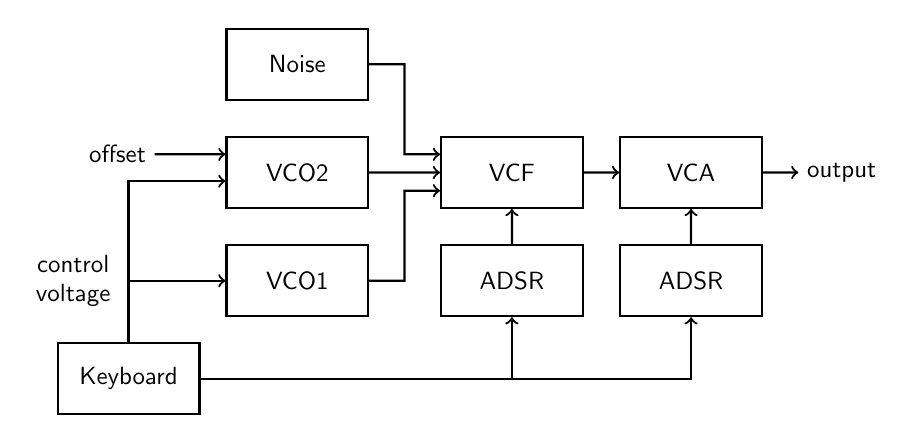
\begin{tikzpicture}[box/.style={rectangle,thick,draw=black,
minimum width=20mm, minimum height=10mm,
align=center,node distance=0.5cm},scale=0.9, transform shape]

\node at (0,0) [box] (noise) {Noise};
\node [box, below = of noise] (vco2) {VCO2};
\node [box, below = of vco2] (vco1) {VCO1};
\node [box, right = 1cm of vco2] (vcf) {VCF};
\draw [thick,->] (vco2) -- (vcf);

\coordinate (coordoffset) at ($(vco2.west)!0.5!(vco2.north west)$);

\node [left = of coordoffset](offset) {offset};
\draw [thick,->] (offset) -- (coordoffset);

\node [right = 1cm of noise] (temp1) {};

\coordinate (vcf1) at ($(vcf.west)!0.5!(vcf.north west)$);
\coordinate (vcf2) at ($(vcf.west)!0.5!(vcf.south west)$);
\coordinate (vco21) at ($(vco2.north east)!0.5!(vco2.east)$);
\coordinate (vco22) at ($(vco2.south east)!0.5!(vco2.east)$);

\node [box, right = of vcf] (vca) {VCA};
\node [box, below = of vcf] (adsr1) {ADSR};
\node [box, below = of vca] (adsr2) {ADSR};

\node [right = 0.5cm of vca] (output) {output};
\node [box, below left = 0.5cm of vco1] (keyboard) {Keyboard};

\node [left = 1.5cm of vco1,align=center](cv) {control \\ voltage };

\coordinate (noisetemp1) at ($(noise.east)!0.5!(temp1.west)$);
\coordinate (vco1adsr1) at ($(vco1.east)!0.5!(adsr1.west)$);

\coordinate (vco2vcf1) at ($(vco21)!0.5!(vcf1)$);
\coordinate (vco2vcf2) at ($(vco22)!0.5!(vcf2)$);

\draw[->,thick] (vco1.east) -- (vco1adsr1) --  (vco2vcf2) -- (vcf2);
\draw[->,thick] (noise.east) -- (noisetemp1) --  (vco2vcf1) -- (vcf1);

\draw[->,thick] (adsr1) -- (vcf);
\draw[->,thick] (adsr2) -- (vca);
\draw[->,thick] (vcf) -- (vca);
\draw[->,thick] (vca) -- (output);

\draw [thick,->] (keyboard) -| (adsr1);
\draw [thick,->] (keyboard) -| (adsr2);
\draw [thick,->] (keyboard) |- (vco1);
\draw [thick,->] (keyboard) |- (vco2.base west);
\end{tikzpicture}
\end{document}
 